\section{Posición}

Para realizar el movimiento de la pelota, es necesario utilizar el vector Up de la pelota guía y multiplicarlo por -1, de forma que el vector resultante mire hacia abajo. Una vez realizado esto, se debe lanzar un rayo para intersecar la superficie, así se obtiene un vector con la posición en la que ha intersecado.

\bigskip

Finalmente, se modifica el valor \textit{pos} de la pelota para que sea igual que el punto de colisión del suelo. Al realizar esto, la pelota aparecerá hundida en el suelo, por lo que es necesario levantarla. Para ello, se debe utilizar el vector normal de la superficie del suelo con la que ha intersecado el rayo y multiplicarlo por el radio de la pelota, para que tenga dicho valor de módulo. Con este vector obtenido, solo es necesario ejecutar el comando \verb|move| en la pelota una vez para sacarla del suelo.

% foto de hundido y despues.
\begin{figure}[H]
    \centering 
	\begin{subfigure}[t]{0.3\textwidth}
	    \centering
	    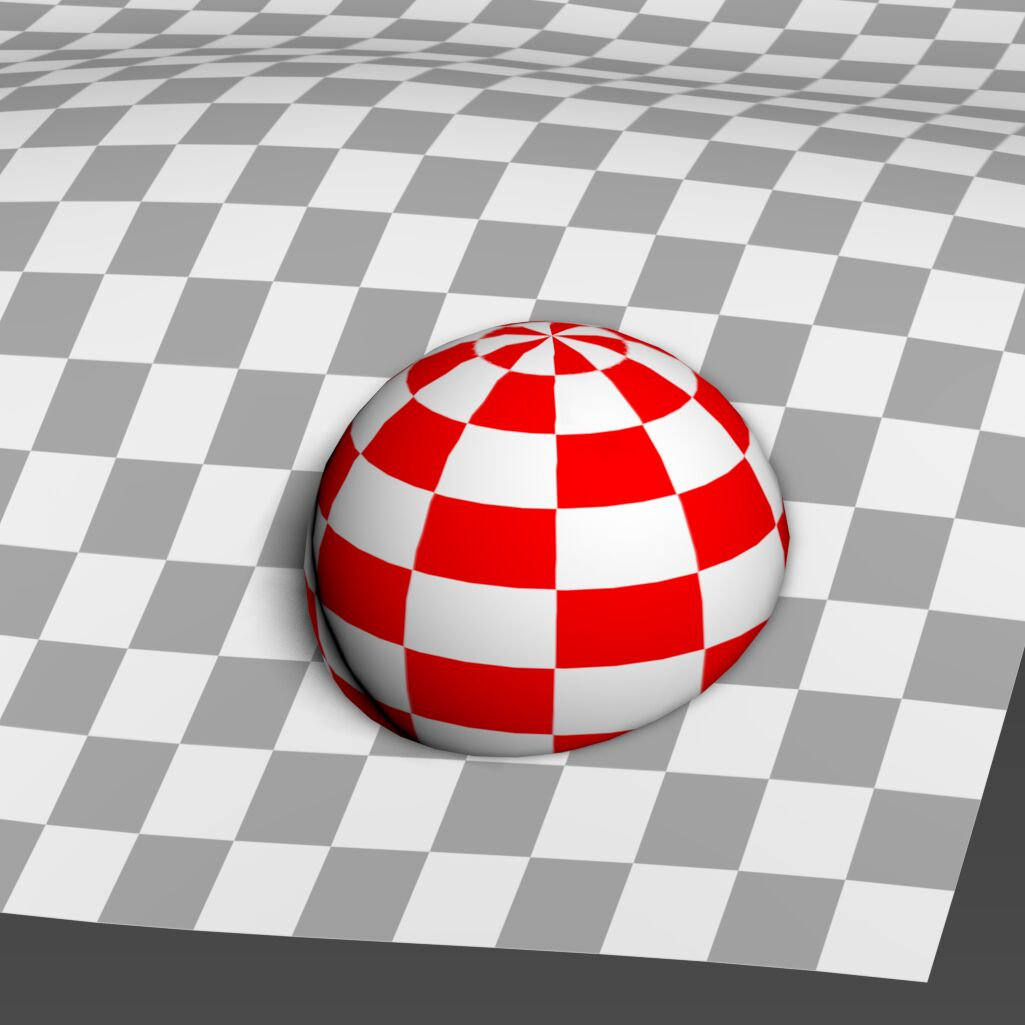
\includegraphics[width=\textwidth]{imagenes/posicion/hundido.jpg}
        \caption{Pelotas hundida en el suelo.}
    \end{subfigure}
    \hspace{20px}
	\begin{subfigure}[t]{0.3\textwidth}
	    \centering
	    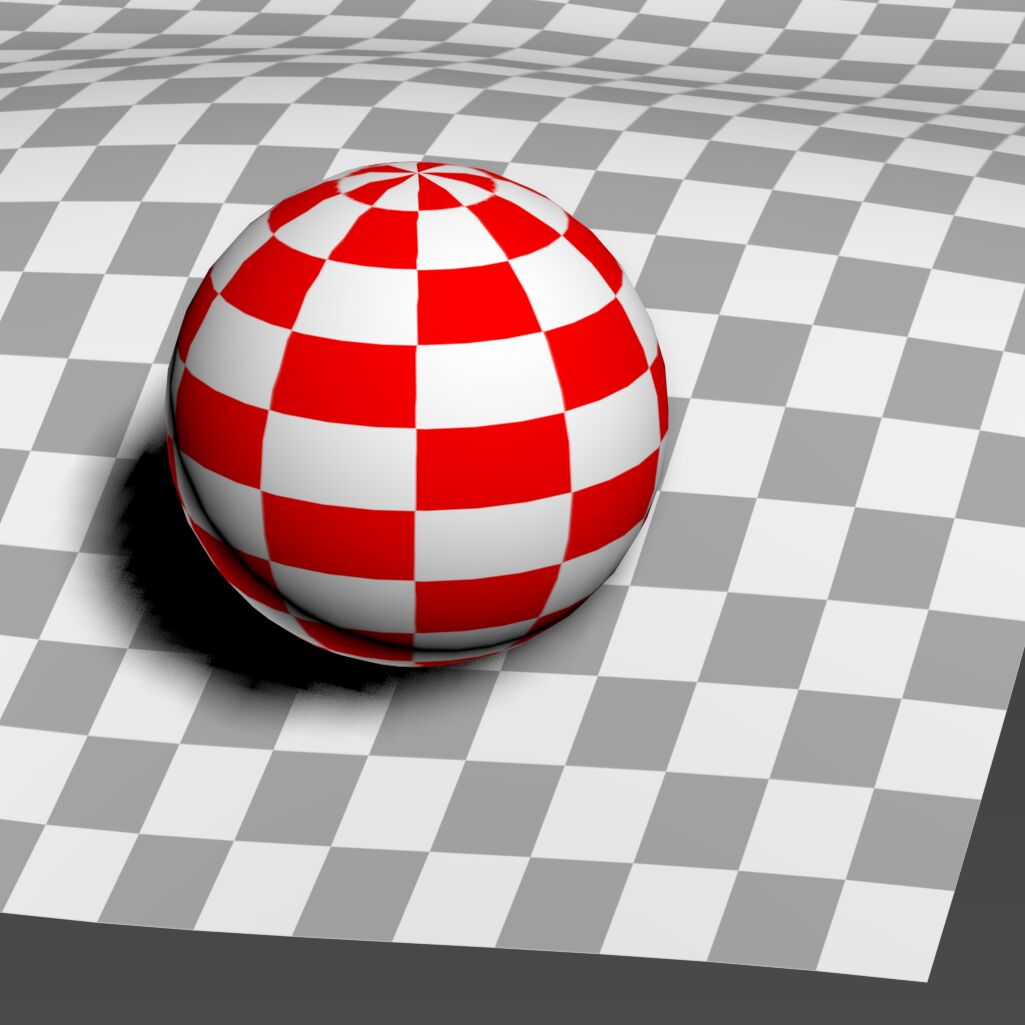
\includegraphics[width=\textwidth]{imagenes/posicion/normal.jpg}
        \caption{Pelotas correctamente posicionada.}
    \end{subfigure}    
    \caption{Diferencia entre usar el comando \texttt{move} y no usarlo.}
\end{figure}

La función para implementar esta funcionalidad es el siguiente:

% codigo
\lstinputlisting[language=MaxScript,firstline=21,lastline=38 ]{../eje_MerloTrujilloAndres_AO_P6.ms}

\bigskip

Y a continuación hay capturas con la pelota en distintos lugares y posicionada correctamente, pero sin rotar, que se hará en la siguiente sección:

% dos o tres fotos de la pelota a distintas alturas.

\begin{figure}[H]
    \centering 
	\begin{subfigure}[t]{0.48\textwidth}
	    \centering
	    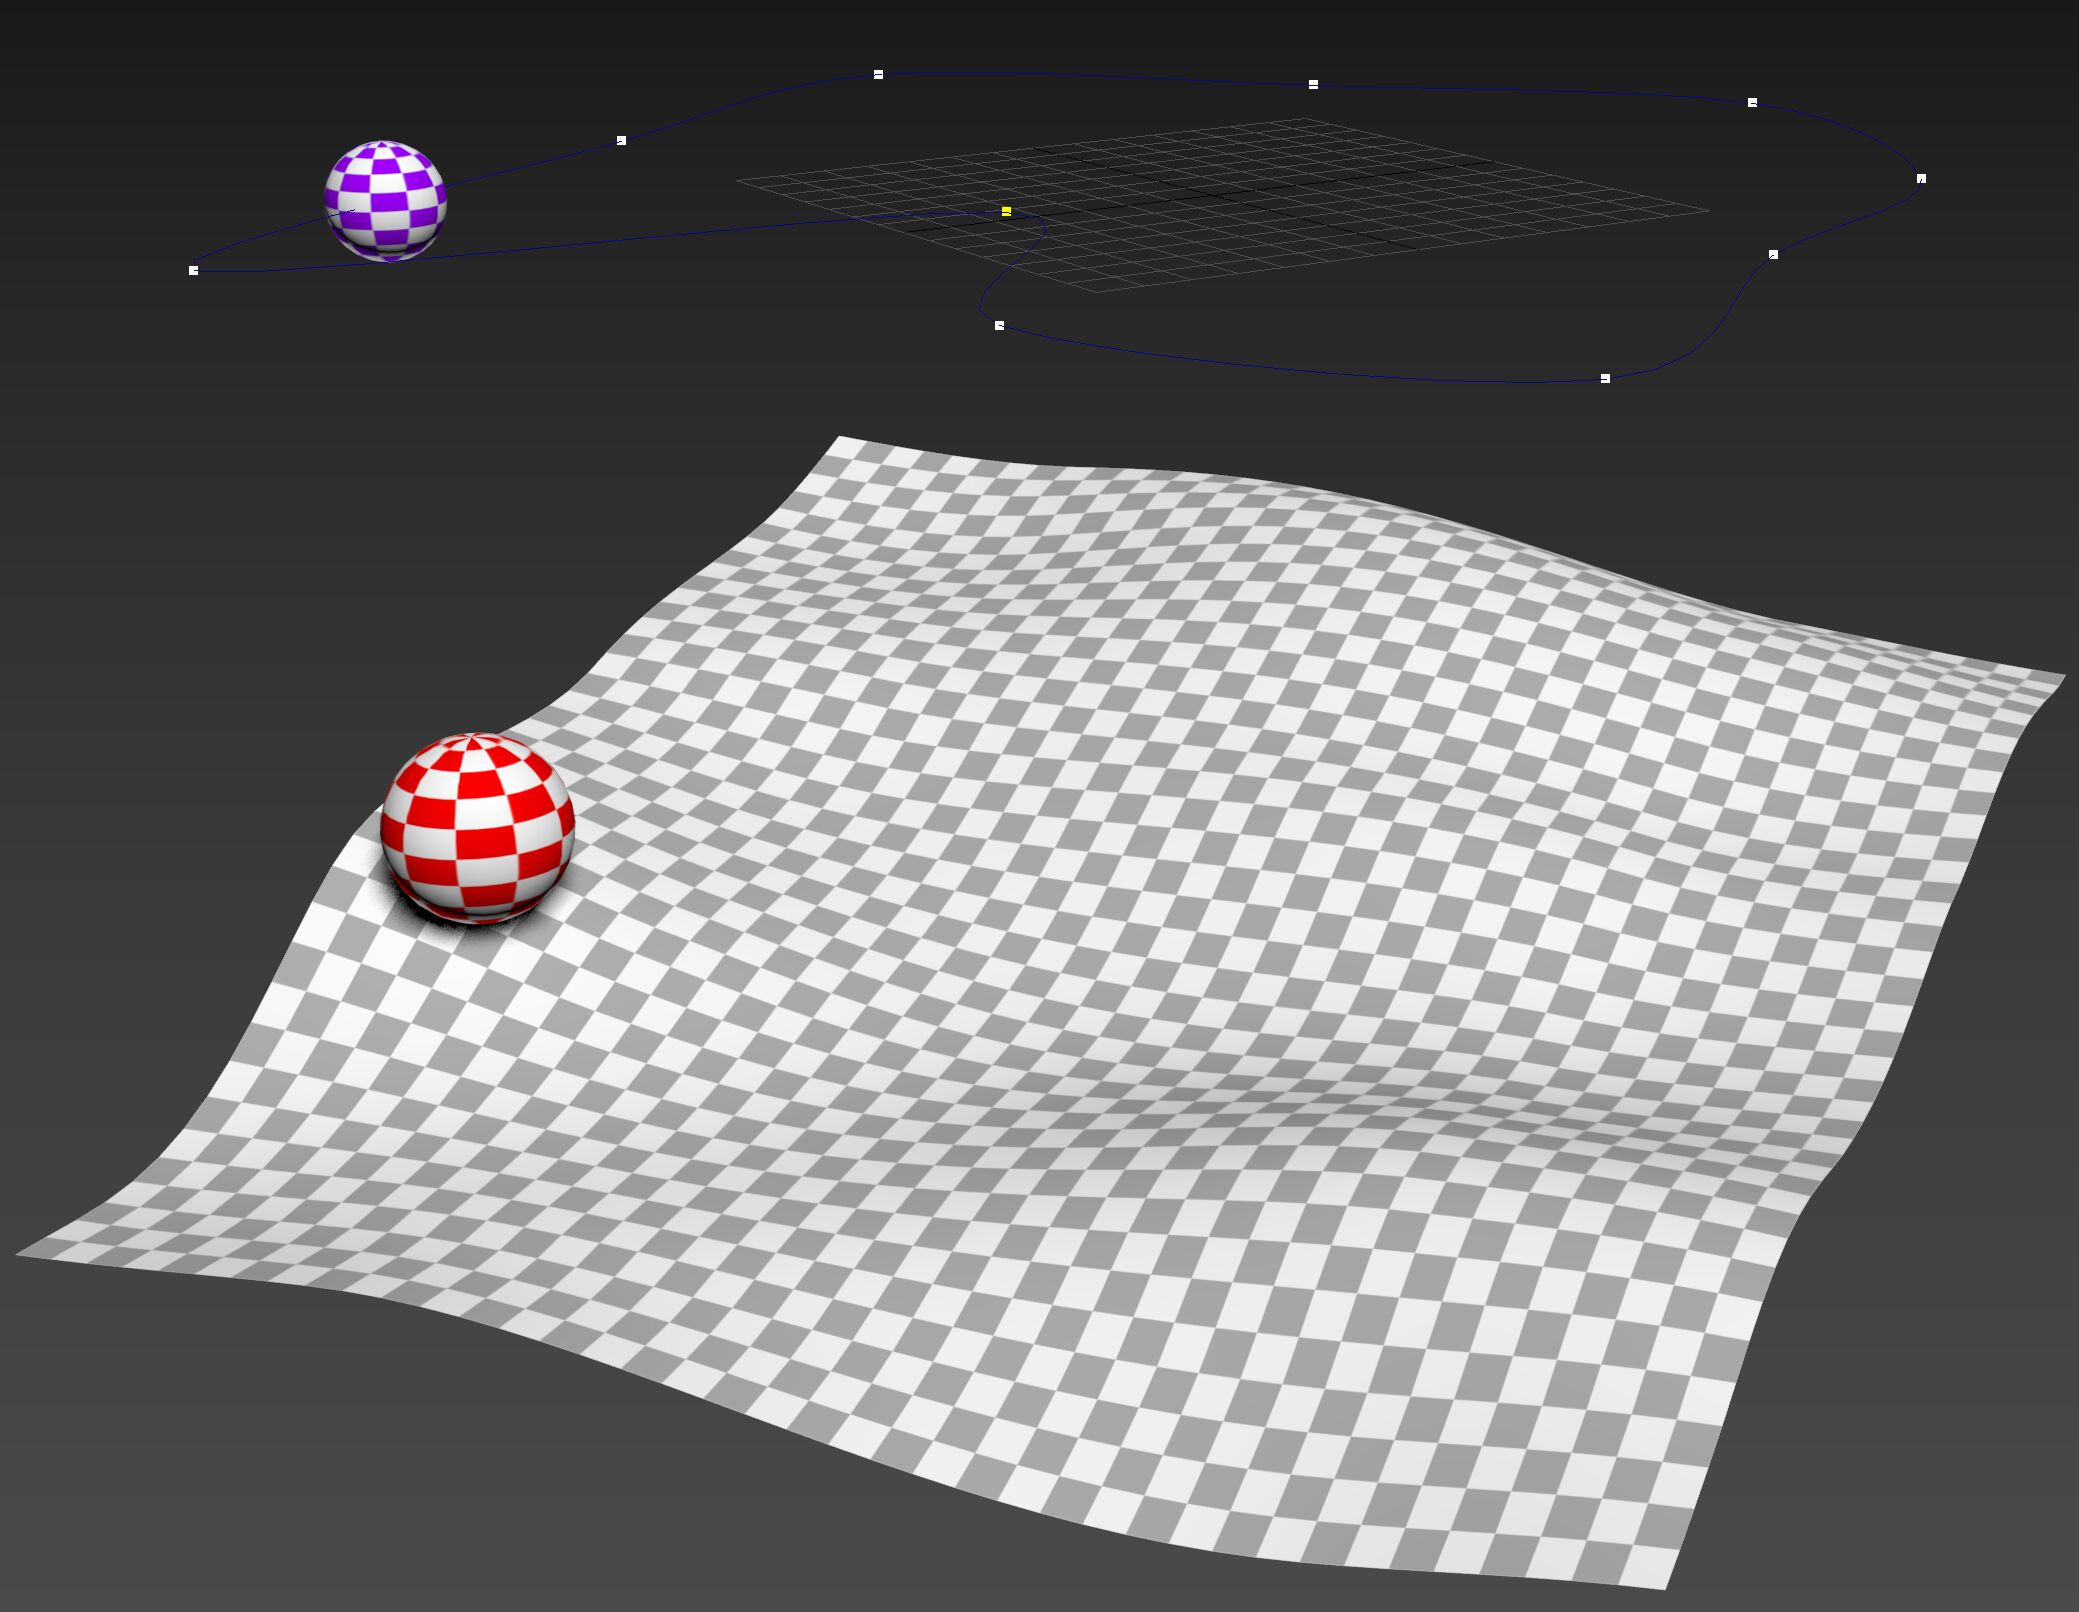
\includegraphics[width=\textwidth]{imagenes/posicion/100.jpg}
        \caption{Pelotas en el instante 100.}
    \end{subfigure}
    \hfill 
    %\par\bigskip %si se desea dejar un margen entre la imagen de arriba y de abajo. SOLO SE PUEDE USAR HFILL O ESTE
	\begin{subfigure}[t]{0.48\textwidth}
	    \centering
	    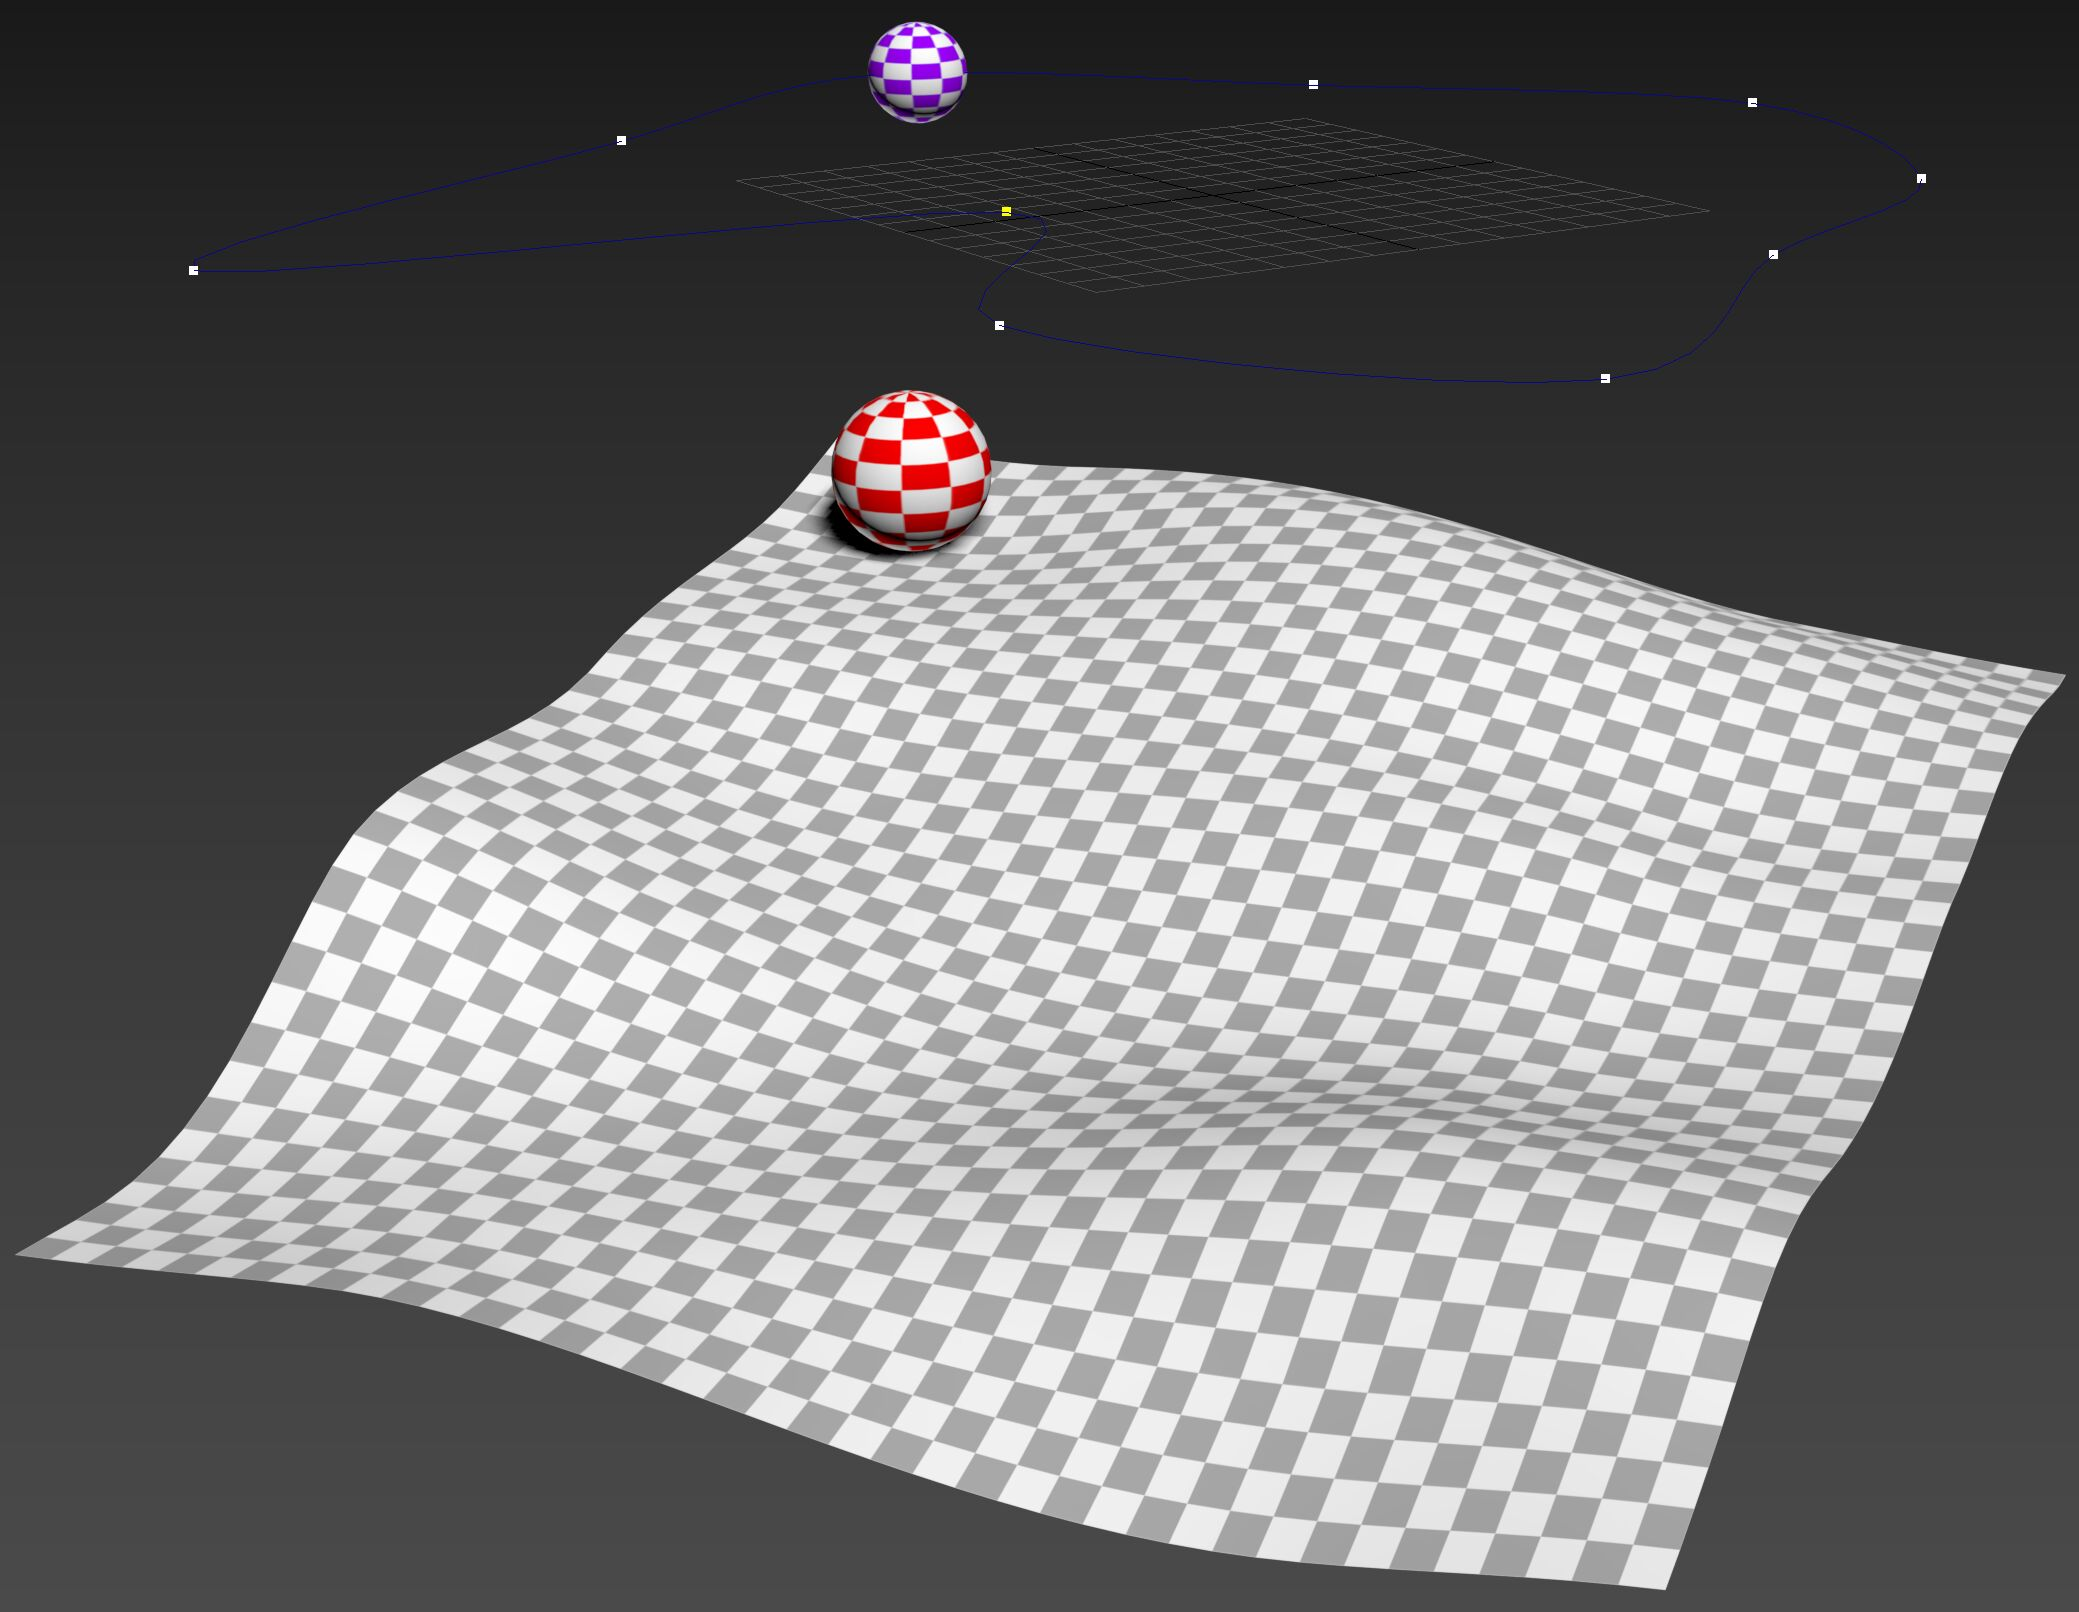
\includegraphics[width=\textwidth]{imagenes/posicion/185.jpg}
        \caption{Pelotas en el instante 185.}
    \end{subfigure}    
    \par\bigskip
	\begin{subfigure}[t]{0.48\textwidth}
	    \centering
	    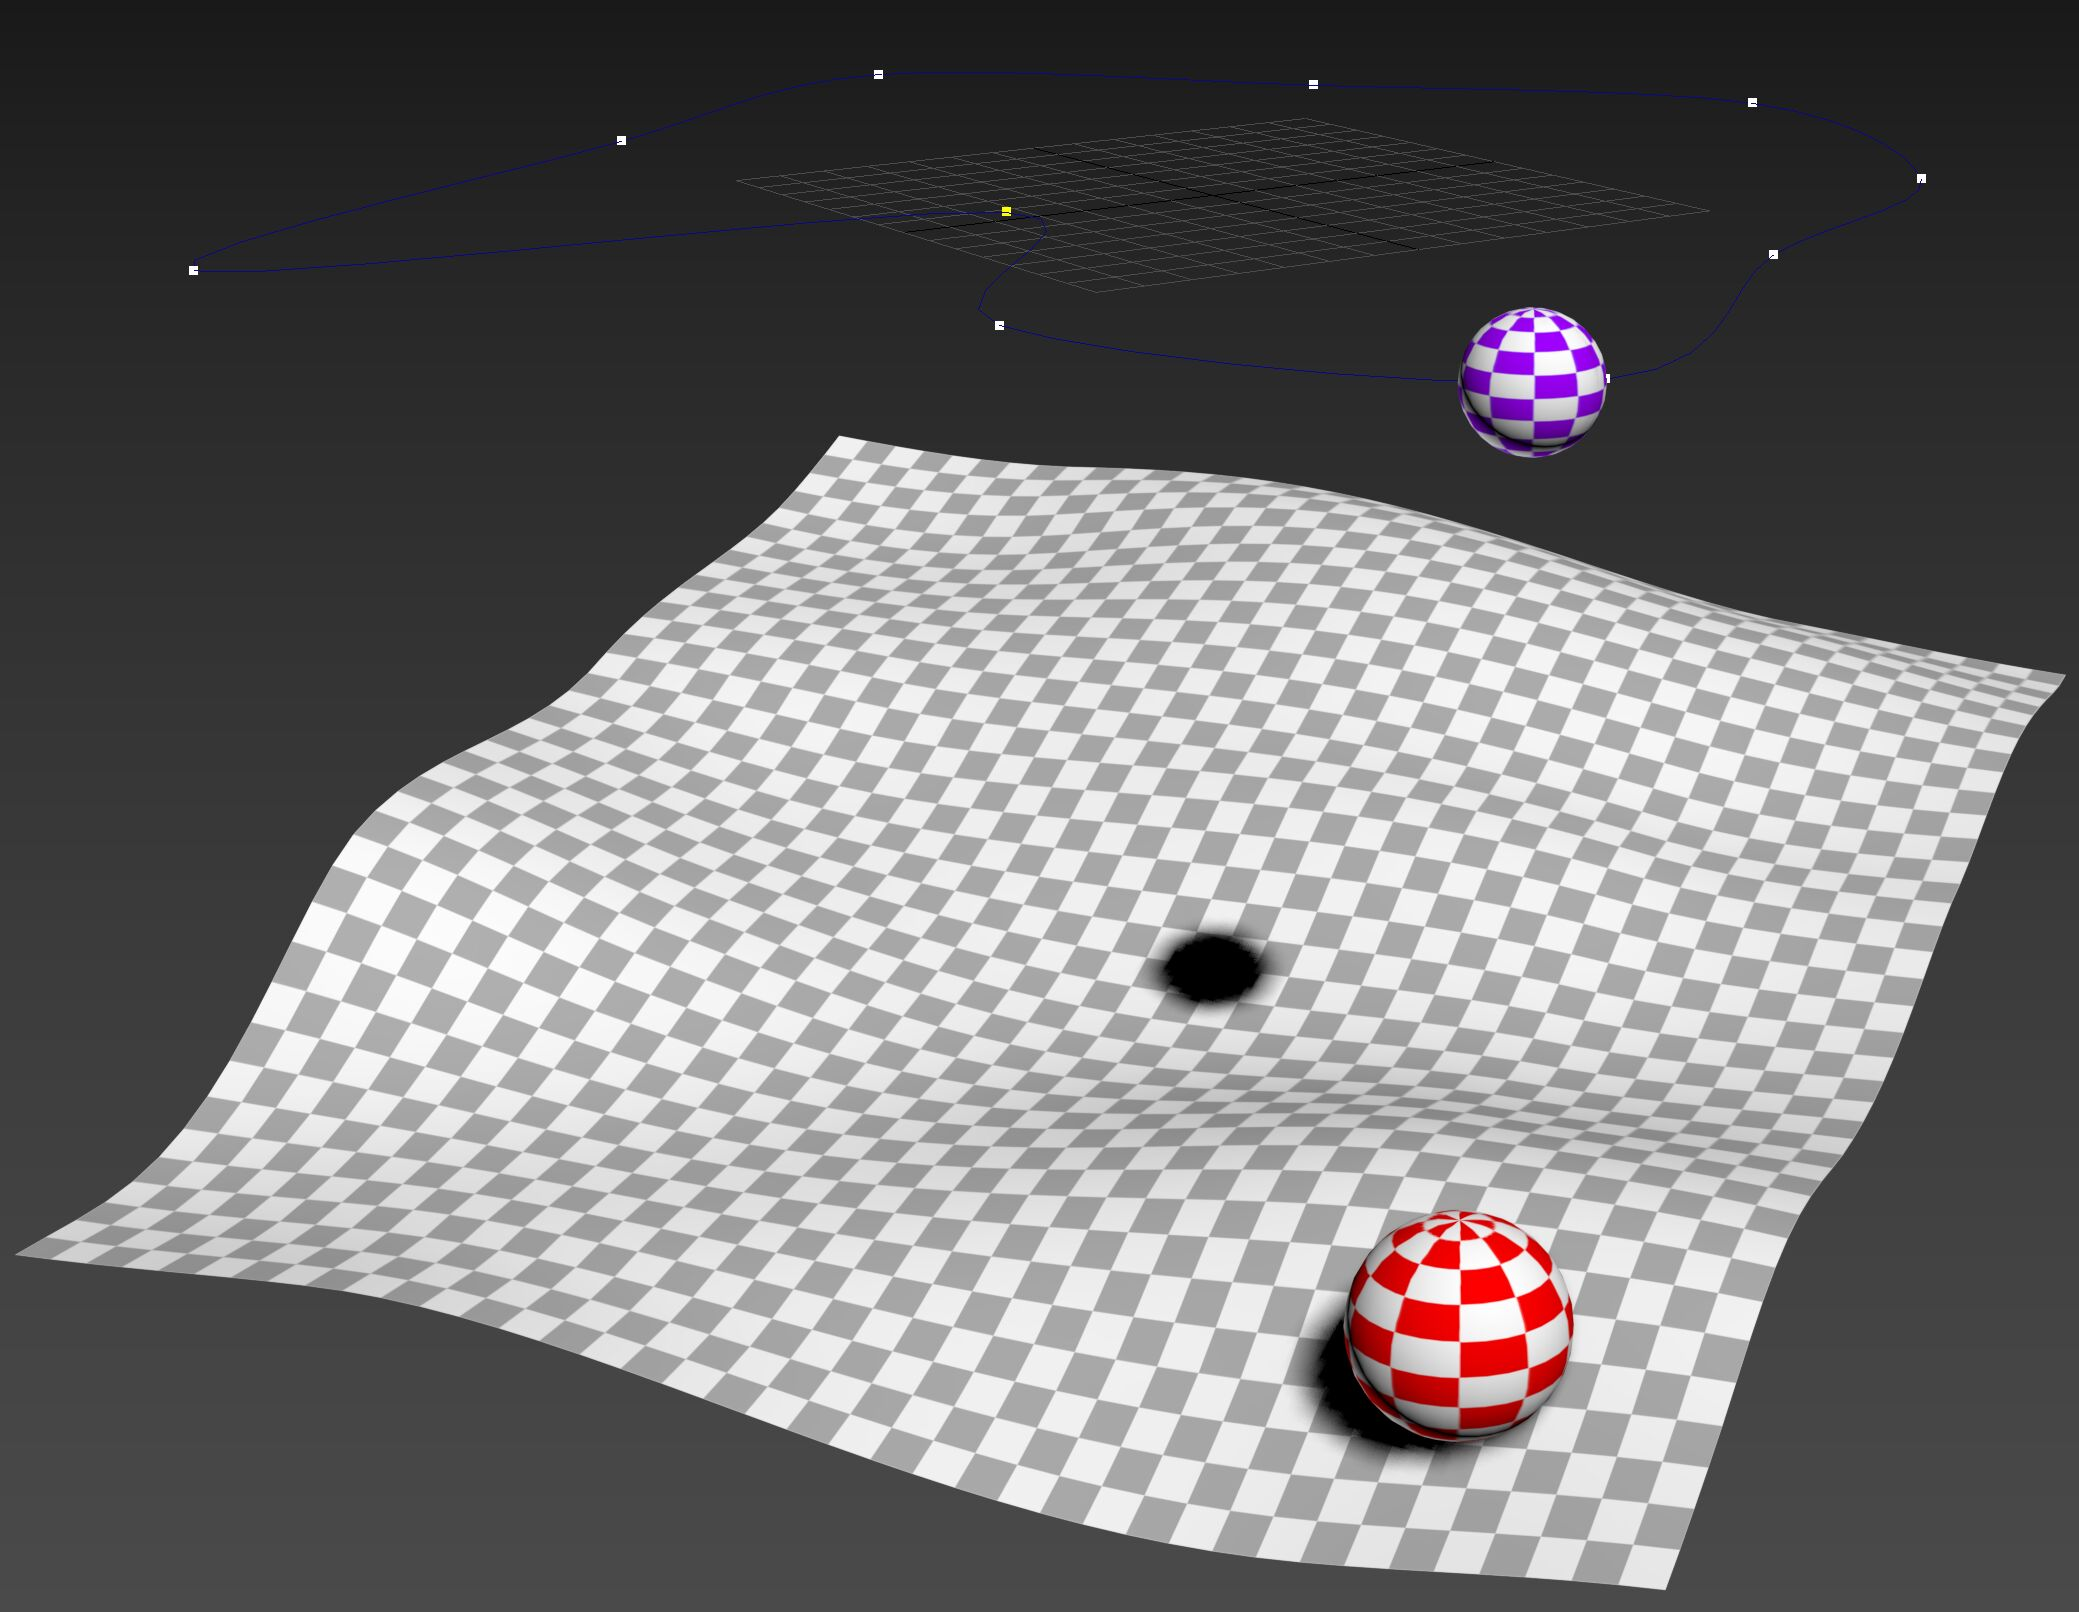
\includegraphics[width=\textwidth]{imagenes/posicion/410.jpg}
        \caption{Pelotas en el instante 410.}
    \end{subfigure}        
    \caption{Visualización de algunos instantes de la animación sin usar la rotación.}
\end{figure}